\chapter{Лабораторная работа}

\section{Цель работы}

Лабораторная работа № 2 выполняется на основе лабораторной работы № 1 и нацелена на освоение возможностей программы Microsoft Project для работы с ресурсами.

\section{Содержание проекта}

Команда разработчиков из 16 человек занимается созданием карты города на основе собственного модуля отображения. Проект должен быть завершен в течение 6 месяцев. Бюджет проекта: 50 000 рублей.

\section{Задание 1: Создание списка ресурсов}

Был заполнен ресурсный лист в соответствии с таблицей.

\begin{figure}[H]
	\begin{center}
		
\includegraphics[width=\textwidth]{imgs/task_1_0.png}
	\end{center}
\end{figure}

\section{Задание 2: Назначение ресурсов задачам}

Было установлено соответствие исполнителям зачач, добавлены фиксированные затраты.

\begin{figure}[H]
	\begin{center}
		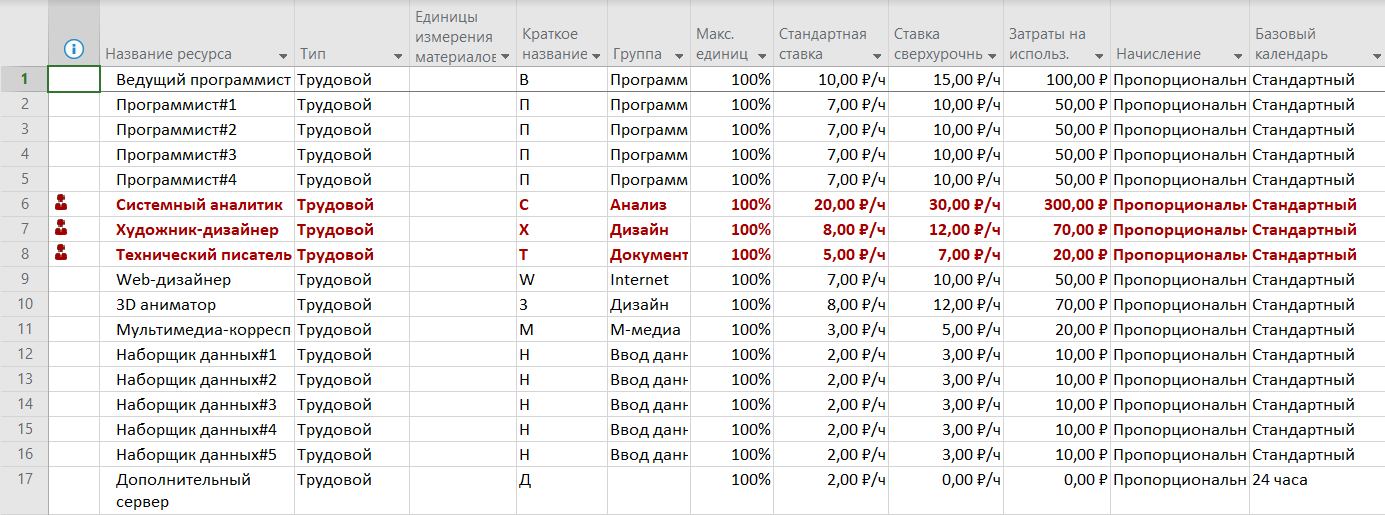
\includegraphics[width=\textwidth]{imgs/task_1_1.png}
	\end{center}
\end{figure}

У исполнителей появились перегрузки из-за того, что они заняты на нескольких задачах одновременно. Продемонстрируем это на оптимизаторе ресурсов:

\begin{figure}[H]
	\begin{center}
		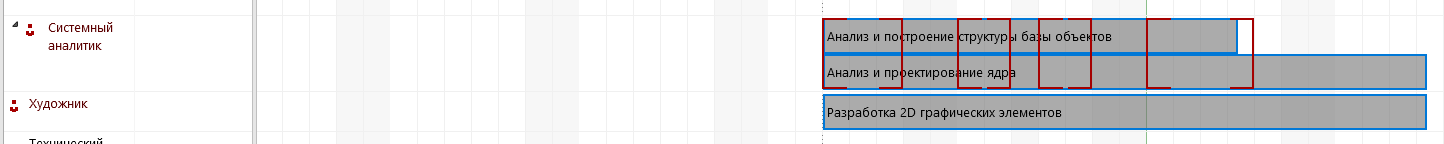
\includegraphics[width=\textwidth]{imgs/task_1_2.png}
	\end{center}
\end{figure}

\begin{figure}[H]
	\begin{center}
		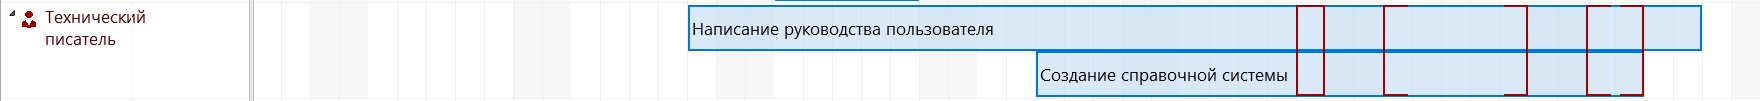
\includegraphics[width=\textwidth]{imgs/task_1_2_1.png}
	\end{center}
\end{figure}

Результаты:

\begin{figure}[H]
	\begin{center}
		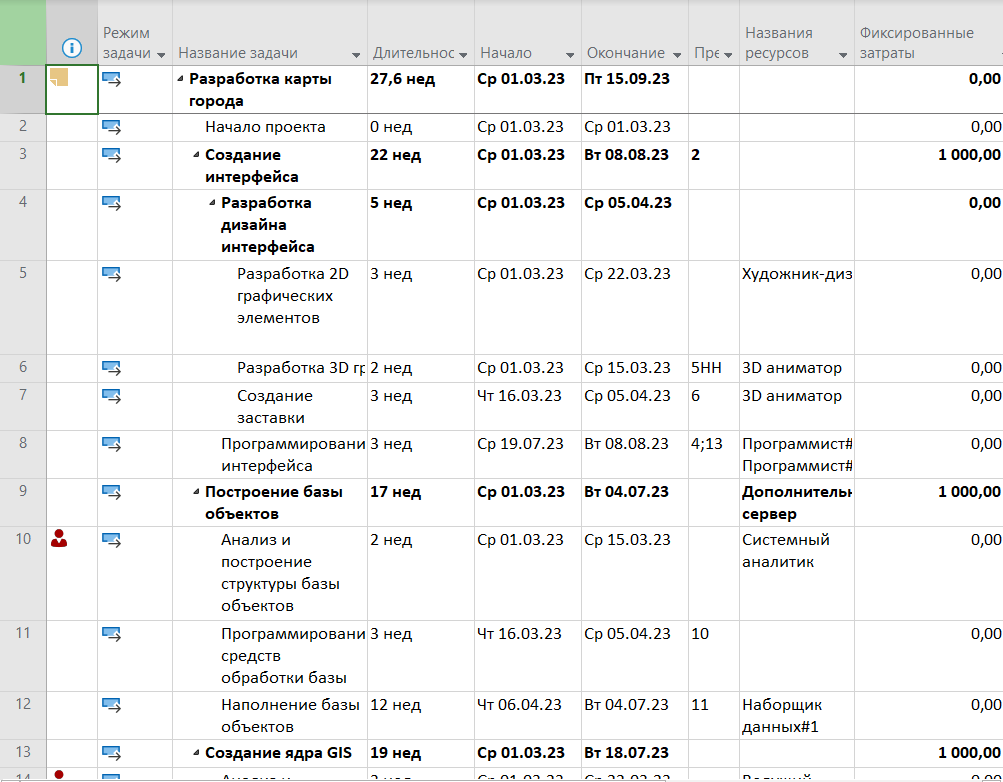
\includegraphics[width=\textwidth]{imgs/task_1_3.png}
	\end{center}
\end{figure}

\begin{figure}[H]
	\begin{center}
		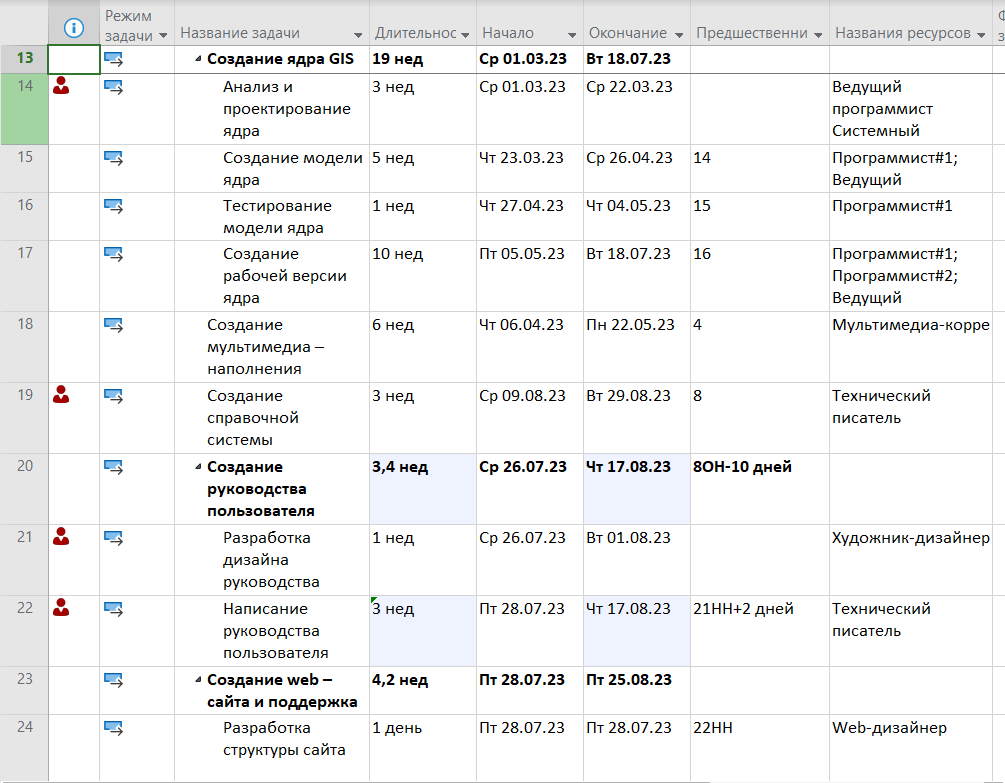
\includegraphics[width=\textwidth]{imgs/task_1_4.png}
	\end{center}
\end{figure}

\begin{figure}[H]
	\begin{center}
		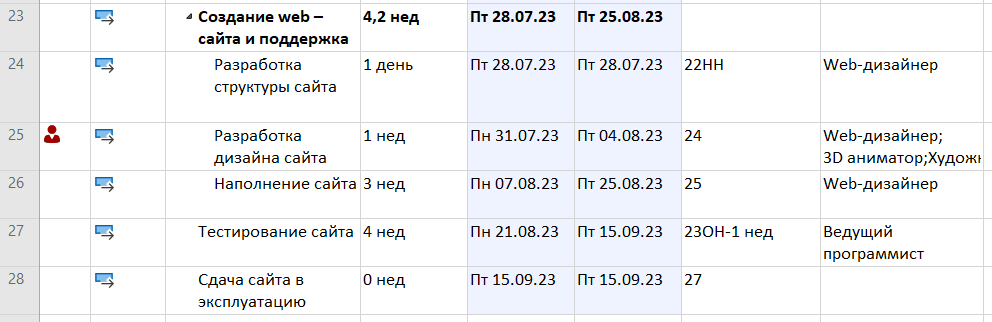
\includegraphics[width=\textwidth]{imgs/task_1_5.png}
	\end{center}
\end{figure}

\section{Задание 3: Анализ затрат по группам ресурсов}

Было просмотренно использование ресурсов, данные сгрупированны по группам.

\begin{figure}[H]
	\begin{center}
		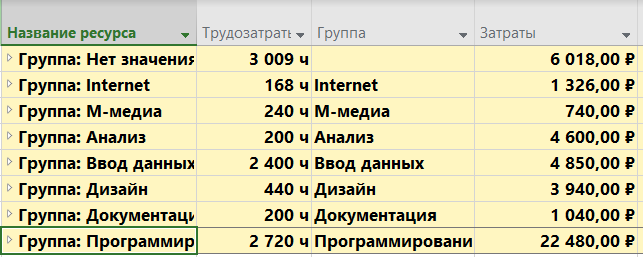
\includegraphics[width=\textwidth]{imgs/task_2_0.png}
	\end{center}
\end{figure}

Вручную было построено два графика:

\begin{figure}[H]
	\begin{center}
		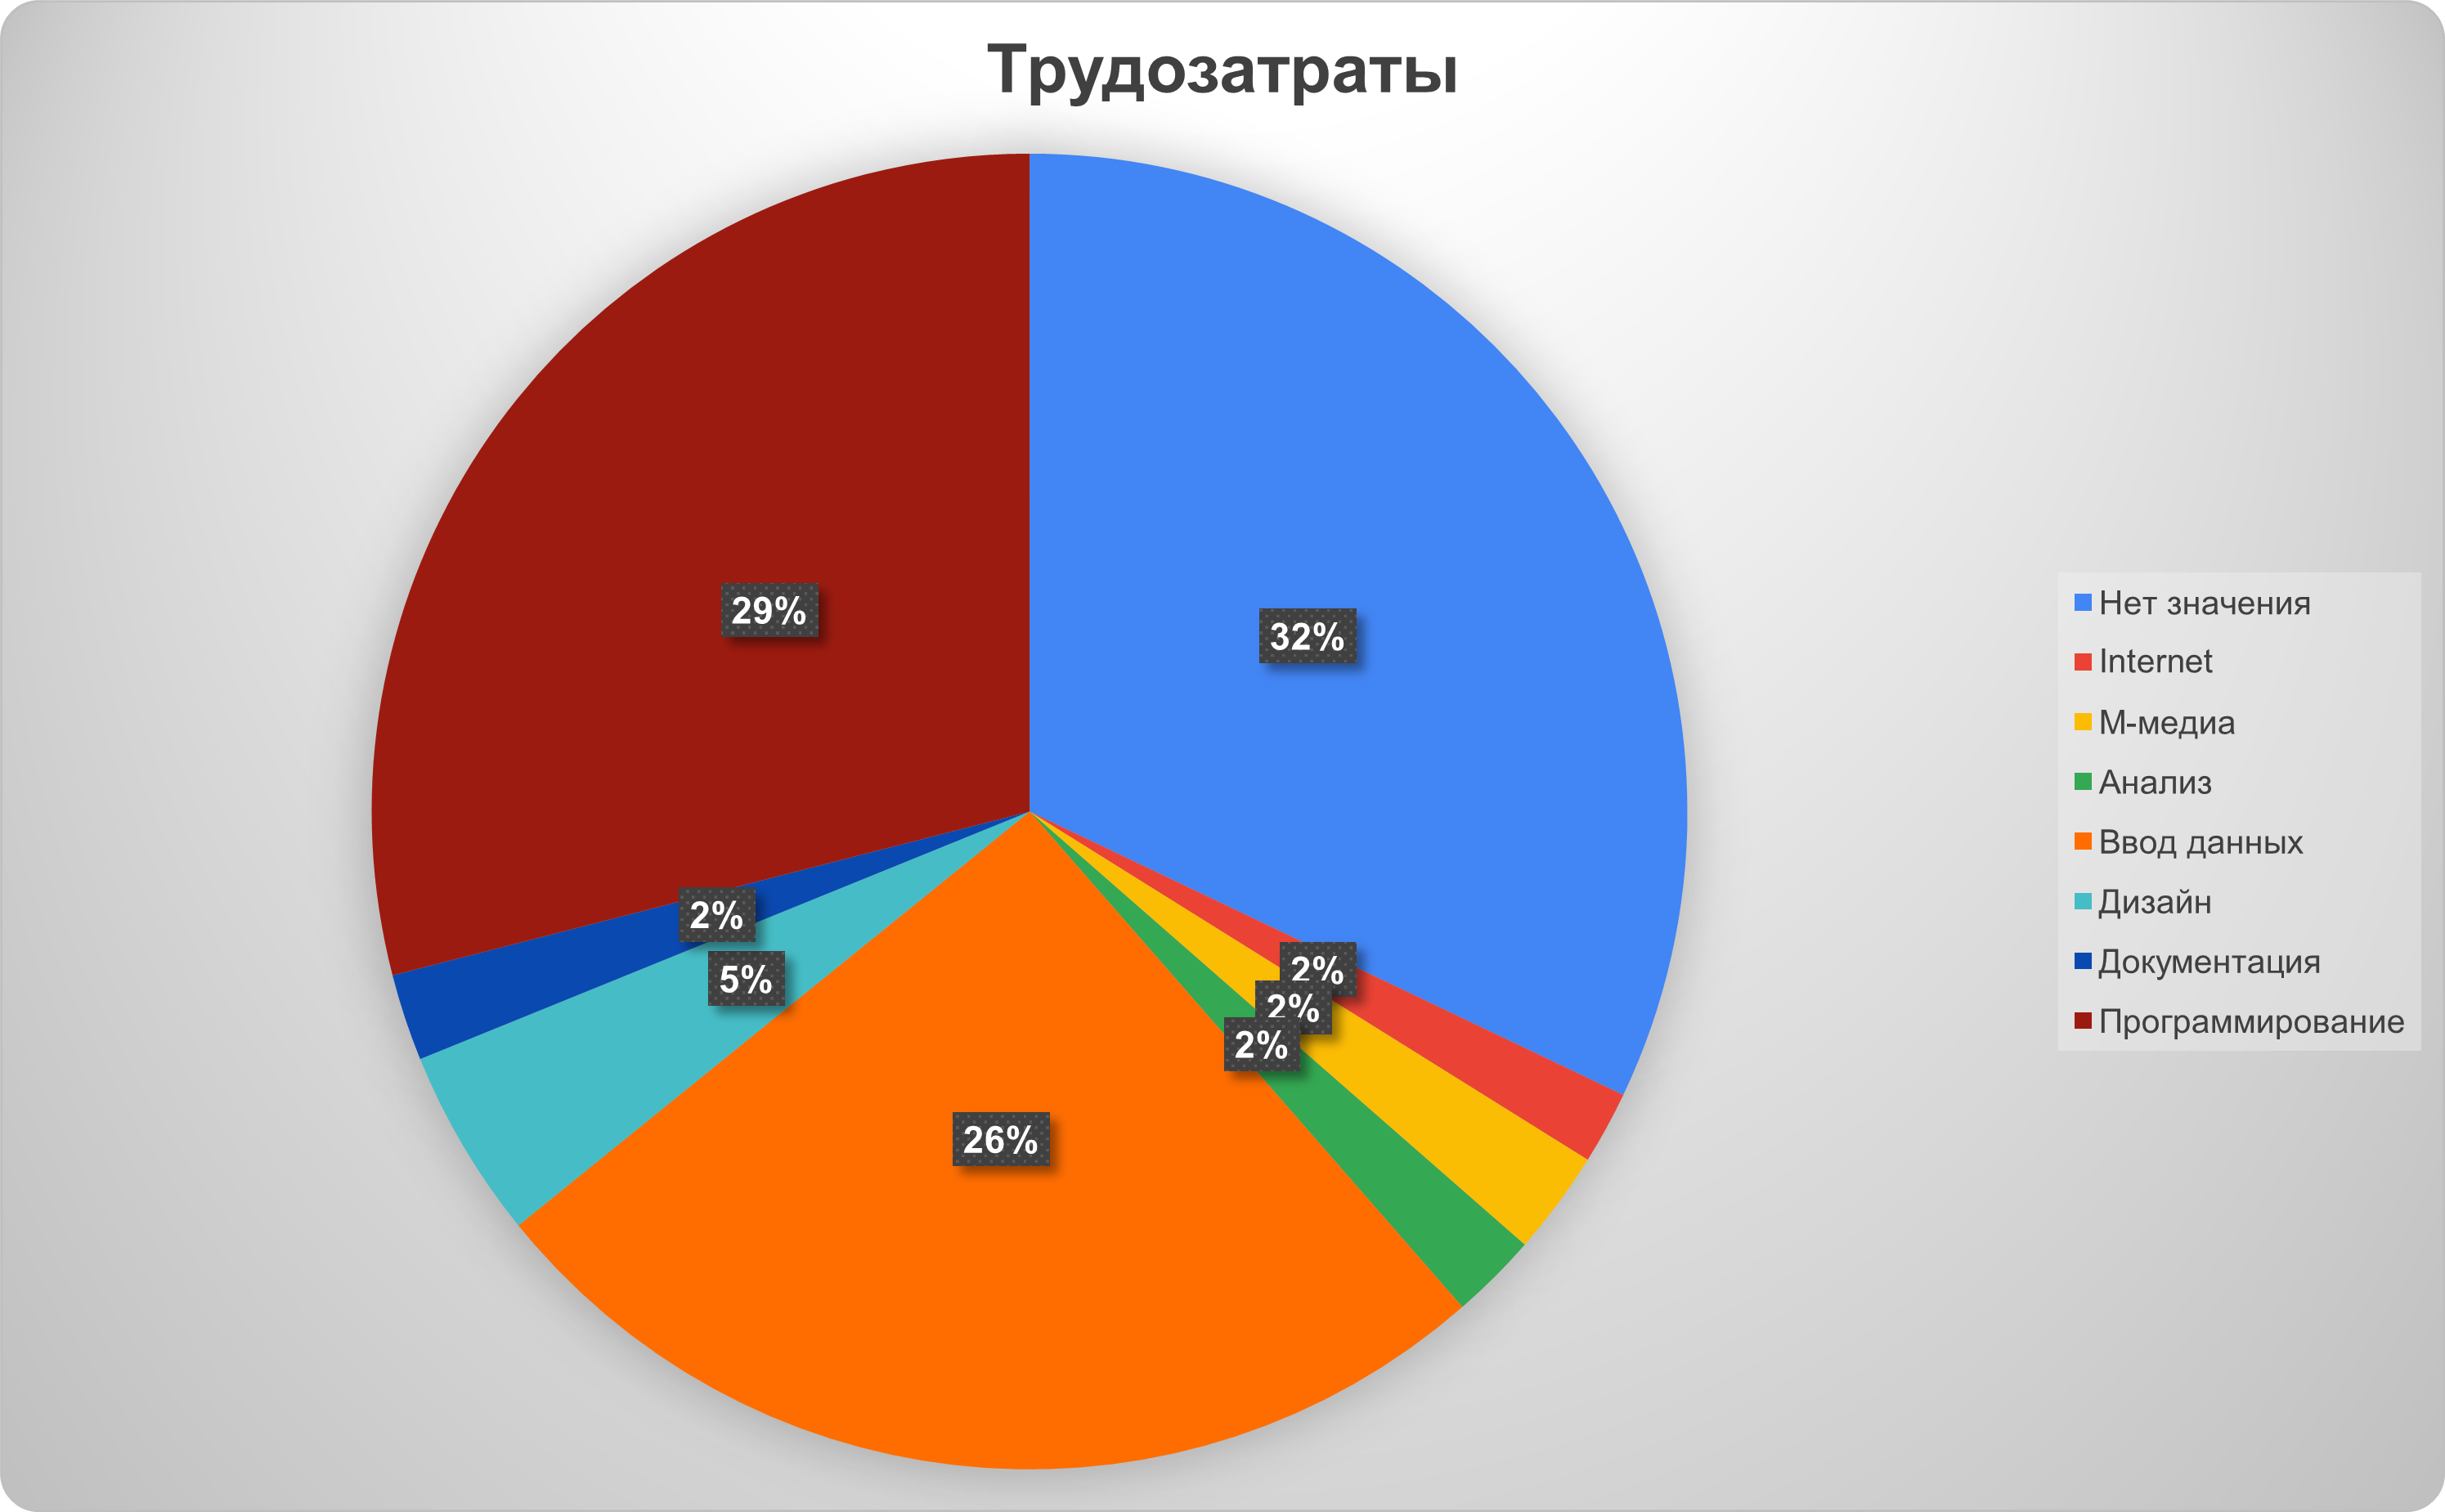
\includegraphics[width=\textwidth]{imgs/task_2_1.png}
	\end{center}
\end{figure}

\begin{figure}[H]
	\begin{center}
		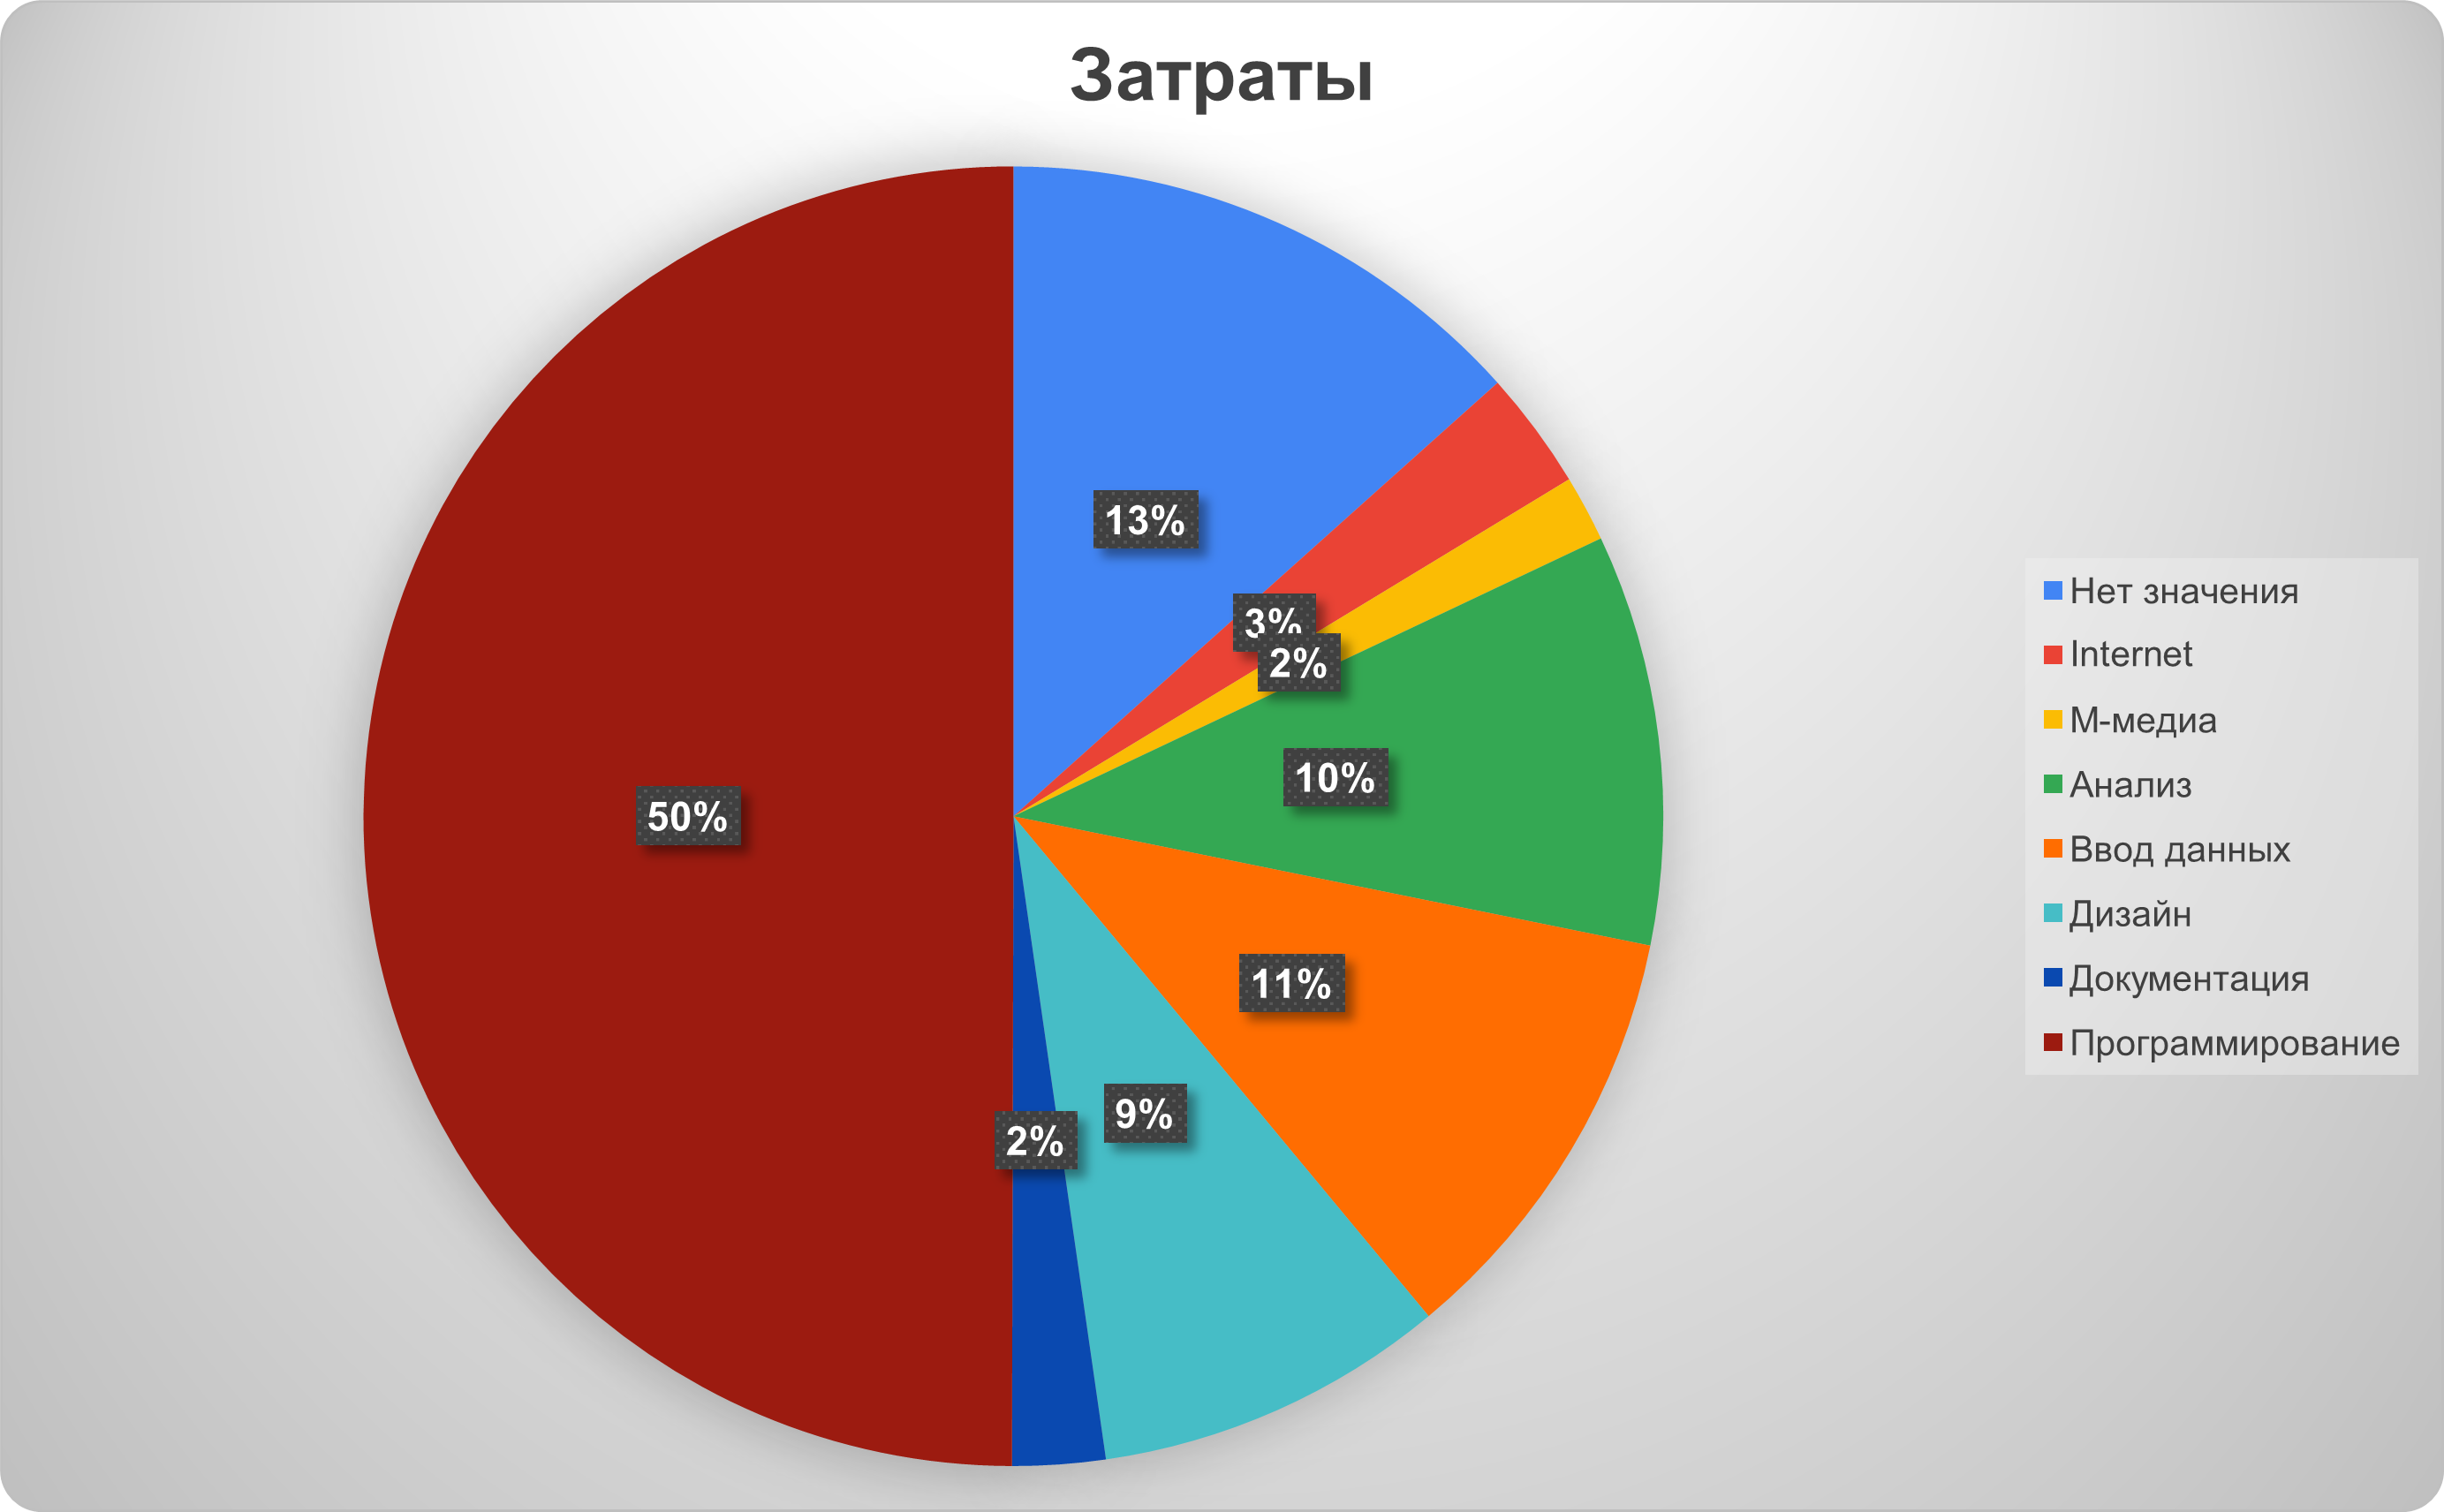
\includegraphics[width=\textwidth]{imgs/task_2_2.png}
	\end{center}
\end{figure}

\textbf{Выводы}

Происходит перегруженность сотрудников, следует решить эту задачу.

Наборщики данных, выполняя 26 \% работы, получают к оплате 11 \% бюджета. Аналитик при всего 2 \% трудозатрат требует 10 \% от всего бюджета. Программисты, выполняя 29 \% работ, требует 50 \% бюджета. Требуется оптимизация ресурсов.